\documentclass[journal,twocolumn]{IEEEtran}

\usepackage{enumitem}
\usepackage{hyperref}
\usepackage{caption}
\usepackage{graphicx}
\usepackage{float}

\title{Evaluating Software Using Black-Box and User Testing}

\author{\IEEEauthorblockN{Oliver Levay, Kristina Sedelius, Adam Tegelberg, Emma Haggren}
\\
\IEEEauthorblockA{\textit{Lunds tekniska högskola} \\
\textit{Lund University}\\
Lund, Sweden \\
(ol1662le-s, kr0363se-s, ad3444te-s, em5261ha-s)@student.lu.se}
}

\begin{document}
\maketitle
\IEEEpeerreviewmaketitle

\begin{abstract}
    This research project compares automated testing, using the software \textit{Cypress}, and manual human testing. This was done by creating three versions of a simple login page as an application and creating a quality assurance checklist relating to the quality attributes described in ISO/IEC 9126. The different versions each had a random set of faults related to the quality attribute requirements that were supposed to be fulfilled according to the quality assurance checklist. After creating the website, tests were written in Cypress using the checklist. The developers that created the website and that wrote the tests had very limited communication to ensure that the tests were not influenced by the implementation. Four tests subjects used the checklist to identify issues with the login page. Automatic testing was more reliable than human testing, a computer will not get tired or have opinions about what is worth testing. The test subjects produced feedback that was never even considered by the research team. Automated tests written in Cypress does not have this ability. The results of the testing showed that the automated tests were more accurate and consistent, but the human testers provided more detailed feedback. Furthermore, the results suggest that a combination of automated tests and human user testing in order to get the best of both worlds. The team was surprised by how well automated testing could find faults in usability.
\end{abstract}

\section{Introduction}
\subsection{Background}
Software quality assurance is crucial to ensure that applications meet user expectations and standards. This project focuses on evaluating a simple login page against the ISO/IEC 9126 product quality standards, which include the attributes functionality, reliability, usability, efficiency, maintainability and portability \cite{ISO}.

\subsection{Objective}
The goal of this research project is to compare automated Black-Box testing with human testing. The automated tests were written in Cypress and both the automated tests and the human tests were guided by a quality assurance checklist. We aim to answer the following research questions:
\begin{enumerate}
    \item What is the overlap between the software quality issues that can be identified by human testers and those that can be identified by automated Black-Box testing? %($A \cap B$)
    \item Which types of software quality problems can only be found by human testers, and which can only be identified by automated Black-Box testing? %($A \setminus B$ and $B \setminus A$)
    \item Which types of issues can't be identified by either method? %($A \cup B)^c$
\end{enumerate}

\section{Method}
\subsection{Software Implementation}
Multiple versions of a simple login page was created using React. The versions were created with intentional issues connected to the ISO/IEC 9126 standards. At first a simple and functioning login page was created, then five new versions were created. Each initial version had a unique focus on exclusively functionality, reliability, usability, efficiency or portability. The introduced issues were:

\textbf{Functionality}:
\begin{itemize}
    \item Faulty logic for login-check, for example not requiring a password, or only being able to log in with admin and no other users.
    \item Password is not case-sensitive.
    \item Enter key disabled for logging in.
\end{itemize}

\textbf{Reliability}:
\begin{itemize}
    \item A pop-up when the login failed, that was irremovable preventing recoverability.
    \item A ten percent probability of randomly failing.
\end{itemize}

\textbf{Usability}:
\begin{itemize}
    \item Non-centered components.
    \item Text with small size, Comic Sans font, and low contrast from background color.
    \item Password- and username-field were switched.
    \item Cursor disappears when hovering over the login button.
    \item Overall visually displeasing.
\end{itemize}

\textbf{Efficiency}:
\begin{itemize}
    \item A delay caused by extremely inefficient search algorithm.
    \item Multiple confirm pop-ups before attempting a login.
\end{itemize}

\textbf{Portability}:
\begin{itemize}
    \item Unable to login on Firefox, Safari and Edge. Only usable with chrome.
\end{itemize}

Maintainability was excluded because it cannot be evaluated with either Cypress or user testing, as it requires analysis of the internal structure of the code. The team that are supposed to write the test cases, and the human test subjects are not supposed to have access to the code rendering the evaluation of maintainability impossible. After the versions were completed they were merged into two versions with mixed issues. The reason for this was so that a tester would not be able to guess which other issues the versions had based on the previously identified issues. For example if a test person notices a pattern of functionality faults and the previous version only had usability faults, they can guess faults without actually testing. The tests were formed so that the faults were random between the different quality criterion.

At the end of the development the final versions were the one original login page, and the two faulty versions. Three users were created with credentials that was communicated to the testing team and the test subjects. The credentials are:

\begin{figure}[h!]
    \centering
    \begin{tabular}{|c|c|}
        \hline
        \textbf{Username} & \textbf{Password} \\ \hline
        admin             & 12345             \\ \hline
        user1             & Password1         \\ \hline
        user2             & Password1         \\ \hline
    \end{tabular}
    \caption{Credentials}
\end{figure}

In addition to the login credentials, the testing team also received a list of elements and their corresponding HTML ID. This was to ensure that the tests would be able to identify the correct element. The elements and their corresponding HTML ID are outlined below.

\begin{figure}[h!]
    \centering
    \begin{tabular}{|c|c|}
        \hline
        \textbf{Element} & \textbf{HTML ID} \\ \hline
        Login Header     & login-header     \\ \hline
        Username Label   & username-label   \\ \hline
        Username Field   & username         \\ \hline
        Password Label   & password-label   \\ \hline
        Password Field   & password         \\ \hline
        Login Button     & login-button     \\ \hline
    \end{tabular}
    \captionsetup{justification=centering}
    \caption{Elements with ID}
\end{figure}

The team that created the website and wrote the automated tests had no further communication related to the code or the tests. The team that created the website had no knowledge of the tests and the team that wrote the tests had no knowledge of the website.

The versions that were tested are outlined below:
\begin{itemize}
    \item \textbf{Version 1}: The original version where all the criteria were met. As seen in figure \ref{v1-2-full} and figure \ref{v1-2-zoom}.
    \item \textbf{Version 2}: A seemingly proper version with hidden issues that included a number of problems, but mainly some functionality and portability problems. As seen in figure \ref{v1-2-full} and figure \ref{v1-2-zoom}.
    \item \textbf{Version 3}: A clearly visually displeasing version focus of this version was to make the site break usability, unreliable, inefficient and without some basic functionality. As seen in figure \ref{v3-full} and figure \ref{v3-zoom}.
\end{itemize}

\begin{figure}[H]
    \centering
    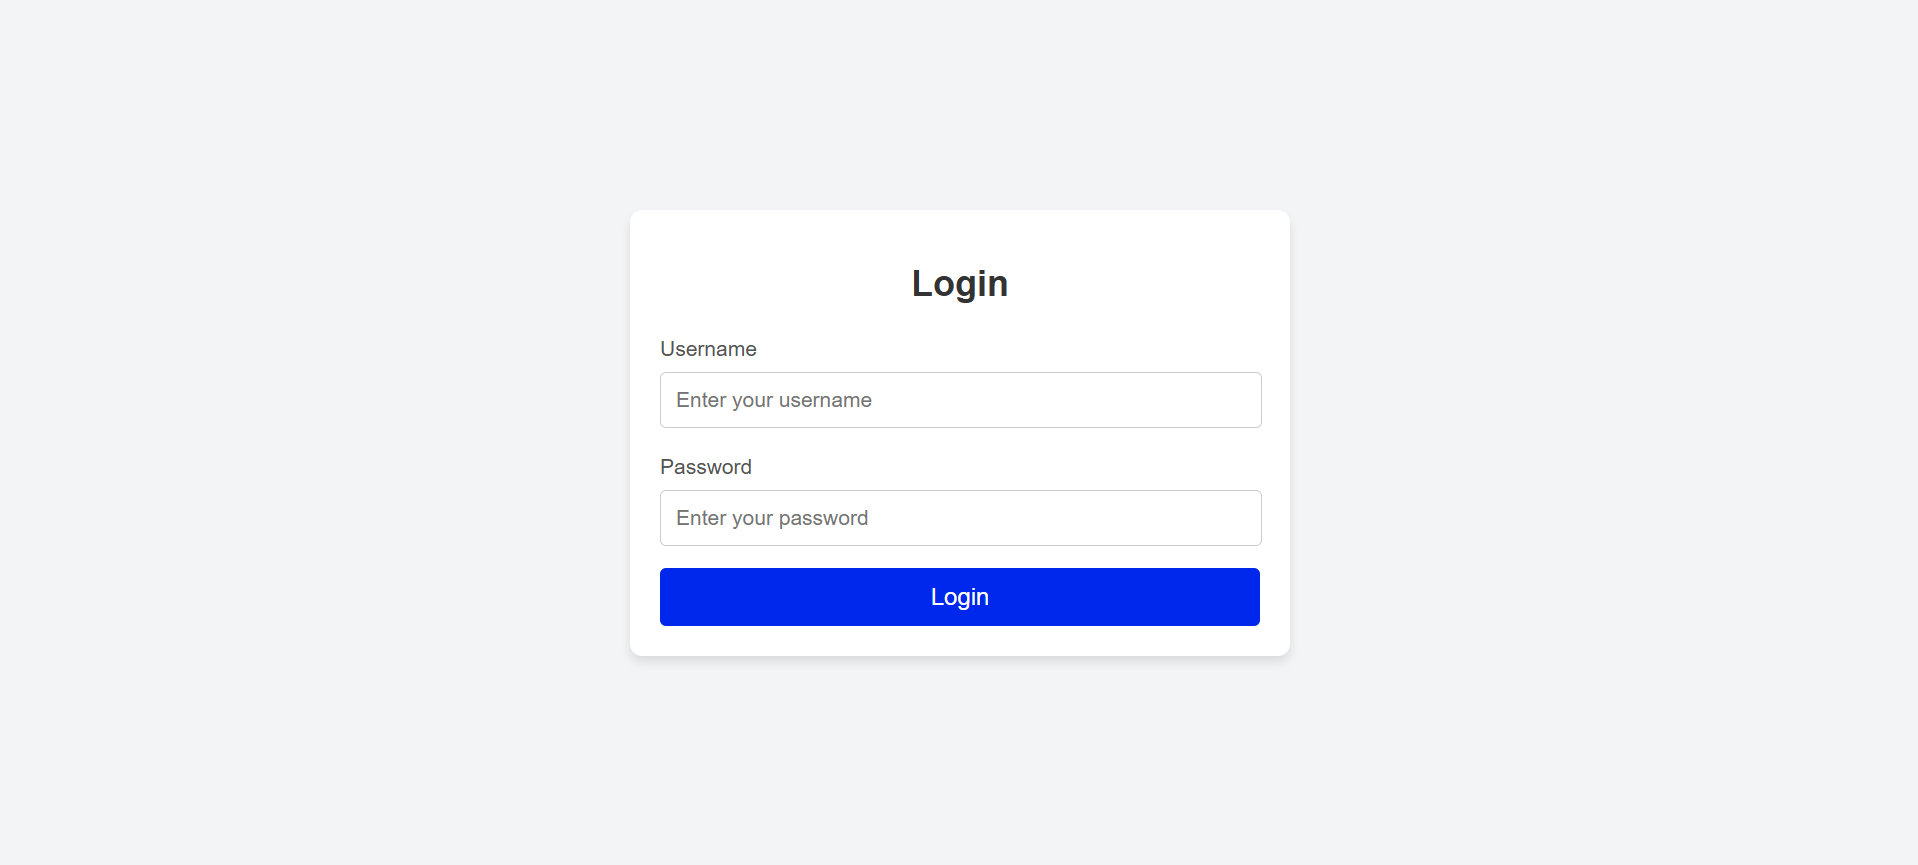
\includegraphics[width=0.6\linewidth]{login-full-size.png}
    \caption{Version 1 and 2, Full sized window}
    \label{v1-2-full}
\end{figure}

\begin{figure}[H]
    \centering
    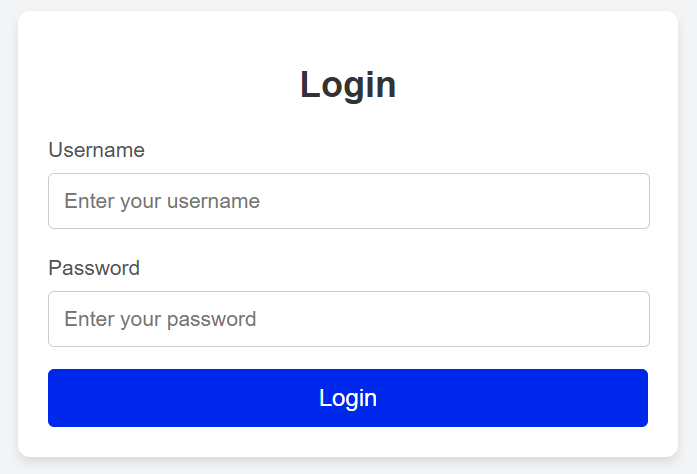
\includegraphics[width=0.6\linewidth]{login normal.png}
    \caption{Version 1 and 2 zoomed into login component}
    \label{v1-2-zoom}
\end{figure}

\begin{figure}[H]
    \centering
    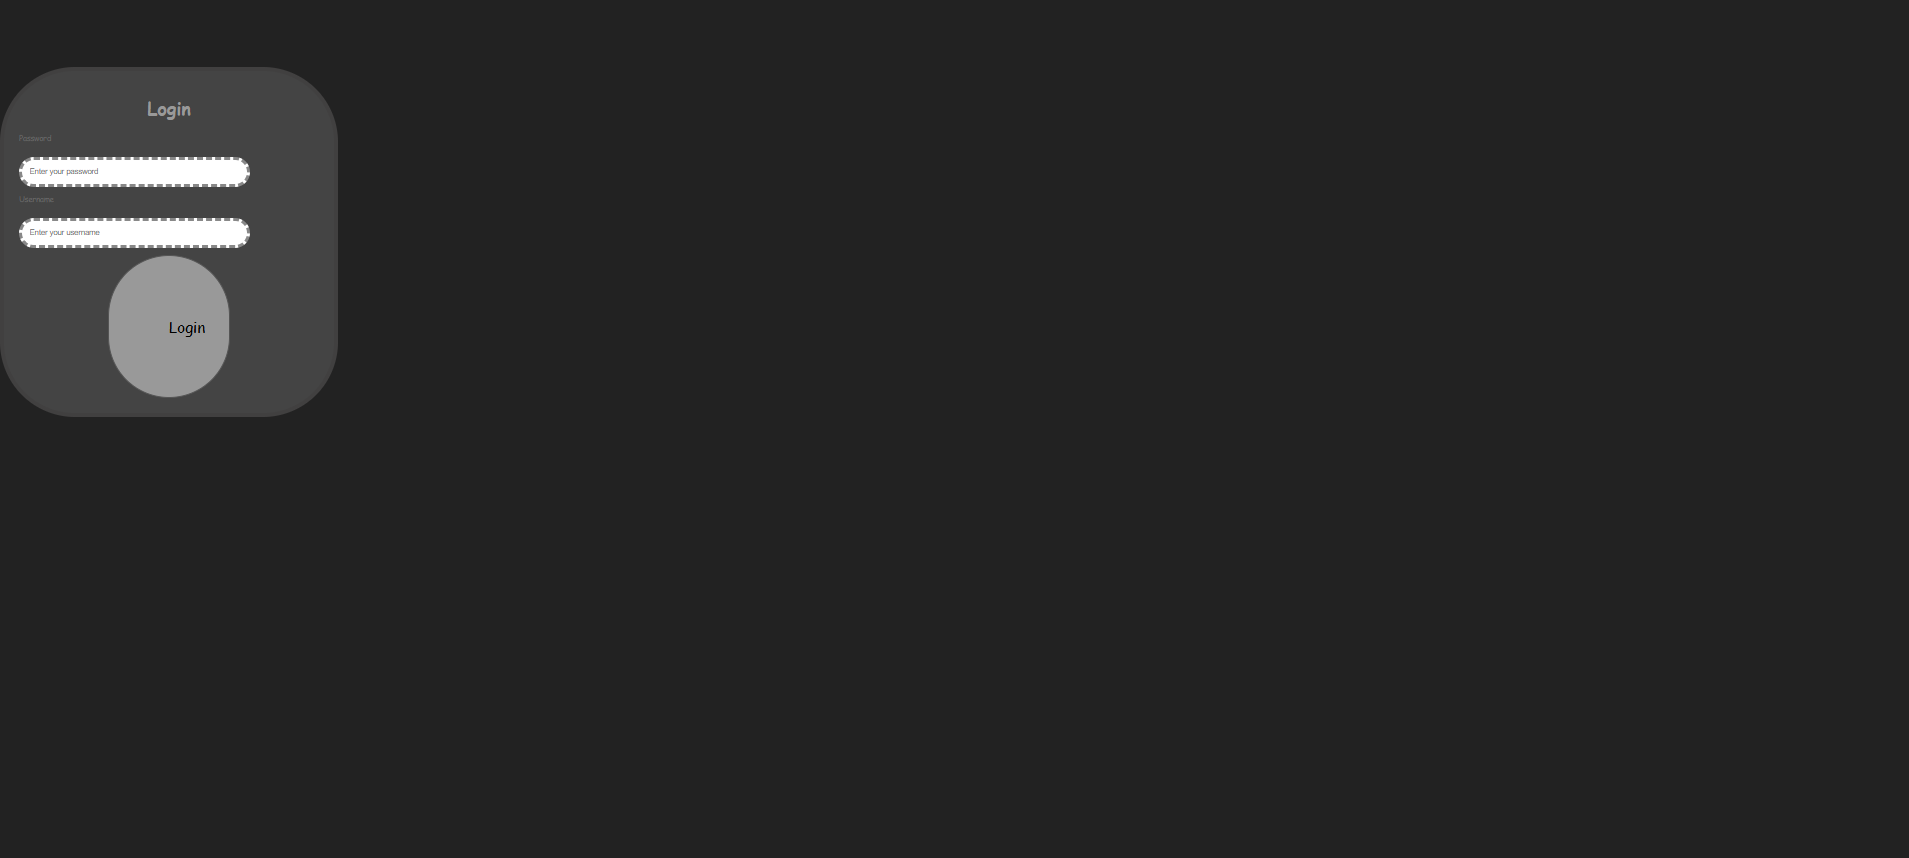
\includegraphics[width=0.6\linewidth]{V3 full size.png}
    \caption{Version 3 Full sized window}
    \label{v3-full}
\end{figure}

\begin{figure}[H]
    \centering
    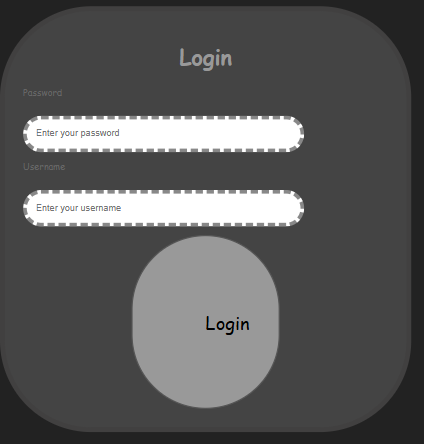
\includegraphics[width=0.6\linewidth]{V3 zoomed in.png}
    \caption{Version 3 zoomed into the login component}
    \label{v3-zoom}
\end{figure}

\subsection{Checklist Development}
%A quality assurance checklist will be developed using sources like \href{https://www.softwaretestinghelp.com/login-page-test-cases/}{Software Testing Help}. The checklist will be categorized using the ISO/IEC 9126 software quality standards.
The quality assurance checklist was developed and categorized using the ISO/IEC 9126 software quality standards and their subcategories.

The checklist included the following criteria:

\textbf{Functionality}:
\begin{enumerate}[label=1.\arabic*]
    \item Verify that a user can log in with a valid username and valid password.
    \item Verify if a user cannot log in with a valid username and an invalid password.
    \item Verify that it says “Invalid username or password!” somewhere for invalid login.
    \item Verify if the data in password field is either visible as asterisk or bullet signs.
    \item Verify if the ‘Enter’ key of the keyboard is working correctly on the login page.
    \item Verify that the login button attempts a login.
    \item Verify that logging in will the take the user to /LoggedIn
    \item Verify that a user that is logged in to the correct account.
    \item Verify that the password is Case-sensitive
\end{enumerate}

\textbf{Reliability}:

\begin{enumerate}[label=2.\arabic*]
    \item Verify that it is possible to log in again after an error.
    \item Verify that logging in behaves the same way every time.
\end{enumerate}

\textbf{Usability}:

\begin{enumerate}[label=3.\arabic*]
    \item Verify that the font is easy to read.
    \item Verify that the contrast of text color and background has a high enough contrast
    \item Verify that the layout of the login page is as you would expect.
    \item Verify that the labels are useful.
    \item Verify that the page is not really ugly.
\end{enumerate}

\textbf{Efficiency}:

\begin{enumerate}[label=4.\arabic*]
    \item Verify the time taken to log in is less than 1 second.
    \item Verify that logging in is not unnecessarily complicated.
\end{enumerate}

\textbf{Portability}:
\begin{enumerate}[label=5.\arabic*]
    \item Verify that the login page works on Google Chrome.
    \item Verify that the login page works on Microsoft Edge.
    \item Verify that the login page works on Safari.
    \item Verify that the login page works on Firefox.
    \item Verify that the login page works on a smartphone.
\end{enumerate}

\subsection{Automated Testing Using Cypress}
Cypress was used to automate tests that evaluate the quality of the login page against the checklist criteria. The tests for \textit{functionality} mostly consisted of simulating writing the username and password and testing if the website behaves as expected.

The tests for \textit{reliability} related to the capability of software to maintain its level of performance over time. This includes recoverability, the ability to recover from errors and reliability compliance where the login page is expected to work the same every time. To test recoverability, tests were made to intentionally produce an error by typing the wrong password and then attempting to log in. Reliability compliance was tested by logging in 50 times.

Usability testing was automated by making assumptions about what it means to have an expected layout and a nice looking website. The assumptions were that an expected layout means that elements should come in the order of username, password and then button. A login website that is "not really ugly" was assumed to have readable text, an expected layout, centered elements and appropriate spacing between elements. The tests that made sure that the elements are centered on the screen also made sure that they were aligned with each other. Label usefulness was tested by making sure that the text above username says something close to "user" and the same for the label describing the password input field.

%% TODO: Describe how the tests turned out in result
% Discuss how writing usability tests was more possible than first expected.
%% TODO: Add suggestions for someone to find out if there's something that is ugly in a way that is not connected to the usability. Are websites ugly because they are hard to use? Or are they hard to use because they are ugly?

Efficiency testing was automated by measuring the time between starting a login attempt and the login screen appearing. In addition to the time it takes for the software to complete its task, tests were also written in a way that ensured that the login process was not too complicated for the user. This was done by ensuring that there were exactly two input fields. If there are more input fields one can assume that the login page is too complicated and time-consuming for the user. Furthermore, the tests ensured that there was exactly one field responsible for the username and exactly one responsible for the password.

Portability was tested by running all the tests again for all the different browsers in the specification.

\subsection{Hypothesis} Before testing began one hypothesis was that some issues, such as subjective usability concerns, would not be detectable by Cypress. Another hypothesis was that humans are error-prone in their nature and that this would hurt their consistency in finding errors across several people. The team were not sure which categories of issues would be hard for a human to test. If a user has a Windows computer testing Safari is exceedingly difficult, but it is not impossible. The research team had an idea that the test subjects would believe it impossible and not attempt to find a solution to this problem.

\subsection{Human Testing with Real Users}
\textbf{Participant Selection}: Four people participated in the testing in total. All test subjects study computer science or information and communication technique at LTH. One of the test subjects participates in the course that this research project is connected to; a course called 'Software Testing' at LTH.

\textbf{Testing Procedure}:
The finished website code was uploaded to a cloud service called Netlify so that the test subjects could display it on their own devices. The test subjects were given a paper with the scenario, a list of the valid login-information and the quality assurance checklist. The participants were then asked to follow the checklist's criteria and evaluate if it was true for the given version of the website. The participants followed through with the checklist for each of the three versions, all the while ticking off what true, and circling what was false. If the test subject was unsure they left it blank.

\section{Results}
\subsection{Test Creation}
Using Cypress to create automated testing turned out to be mostly straightforward and not too complicated. There were a few hurdles that we had to overcome.

\begin{enumerate}
    \item Cypress does not support Safari. There is experimental support for Safari using the open source browser engine WebKit which Safari is built upon. This means that the tests are not run in the actual Safari browser. This could potentially lead to differences in how the website is displayed and how the tests are run.
          % DISCUSS, it turns out that WebKit has the same user agent as Safari when running tests in Cypress and they should have the same functionality since Safari is built on WebKit.
    \item The usability tests had a lot of complicated code to compare layout alignment, ordering and color contrast. Cypress does not natively support this kind of testing. Testing how long something takes or simulating pressing a key on the keyboard for example has native support which makes that kind of testing easy and efficient. Usability testing turned out to be possible but not easy.
          %% Discuss: Cypress does not have native support for this kind of testing because the assumption that we have, that Usability testing with automated programs is unneccessary if not impossible, is held by a lot of other people. 
\end{enumerate}

The test code is available in its entirety in the appendix bajs. %%todo reference correctly

\subsection{Automated Testing Results}
The results from running the test have been compiled to 4 reports, one for each browser supported. The reports are available at appendix bajs. %%todo reference correctly
After the test reports were compiled the team used them to determine the checklist validity. The research teams interpretation of the results are outlined in its entirety in appendix bajs. %%todo reference correctly
In order to compare automated testing with human testing the results from both are compiled in a Google Sheets document available in appendix bajs.
The accuracy of the answers are outlined below.
\subsubsection{Fully functional}
All tests passed which lead the team to believe that all the requirements are fulfilled. This was also the correct answer according to the keys that the team had prepared before initiating testing.

\subsubsection{Mostly reliability and portability issues}
Checklist item 3.1 \textit{Verify that it is possible to login again after an error} was incorrectly marked as TRUE. In the testing code an error is produced by attempting to enter an incorrect password, but in this version every password is correct, so no error is produced. This issue would be remedied by creating a test that produces an error by entering an incorrect username as well.
% DISCUSS: One could argue that it can be marked off as not relevant because other test cases concluded that users can log in with any kind of password making it irrelevant if the user can log in again after an error.
% DISCUSS: Even if the error would be irrelevant it still is a good testament to how the writers of the tests will have inevitably errors in the code because of unforseen circumstances. 
% DISCUSS: Humans made the same mistake

\subsubsection{A lot of issues}
Surprisingly version 3 that we thought would be difficult for the automated testing suite to evaluate did not have any mistakes. The tests would suggest that the labels are useful because it says "Username" and "Password" on them. The tests show that the font is not a usual one and the font size is too small, and the contrast is bad and hard to read. The team made the call that the labels are not useful based on this information.

% What is the overlap between the software quality issues that can be identified by human testers and those that can be identified by automated Black-Box testing? %($A \cap B$)
% Which types of software quality problems can only be found by human testers, and which can only be identified by automated Black-Box testing?
% Which types of issues can't be identified by either method? %($A \cup B)^c$

In summary all the issues that we set out to test \textit{can} be identified with automated testing. % discuss how some are harder to identify than others, is it worth it to write tests for?
Therefore, the answer of question 3, is no. There are no type of issues that cannot be identified by either automated tests or human testers because automated tests \textit{can} identify all types of issues we set out to find.

\subsection{Human Testing Results}:
The results from the human testing was inconsistent, but all issues had at least one correct answer from one of the test subjects. The humans were terrible at identifying Portability issues because if they did not have the browser requested they did not make efforts to test it on a friends computer or install a new browser. Some test subjects assumed that it would work on the other browsers because they could not be bothered to test it out, or did not answer. Other test subjects mistakenly assumed that the site worked on a given browser because it loaded correctly. If they had attempted to log in they would find out that it does not work. The automated tests ran by the computer had no issue running all the tests again with a different browser. Boredom and laziness is not a factor for the computer. For version 3 one test subject could not log in because they did not try the admin account which gave wildly inaccurate results and tracking the biggest fault would be difficult. The computer did not have any issue logging in with each account. %% Discuss: Motivation was low for the test subjects to follow the instructions thoroughly, probably because they are not paid to do this. Paid QA testers would probably do a better job. The computer does not require payment to do as they are told.

\subsection{Analysis of Overlap and Differences}
\textbf{Union (A $\cup$ B)}: Issues found at all. \\
\textbf{Intersection (A $\cap$ B)}: Issues found by both methods. \\
\textbf{Unique to Cypress (A \textbackslash B)}: Issues only detected by automated testing. \\
\textbf{Unique to Human Testing (B \textbackslash A)}: Issues only identified by human testers. \\
\textbf{Union complement $(A \cup B)^c$}: Issues not found.


\section{Discussion}
\subsection{Interpretation of Findings}
%Here we will discuss the overlap and differences between the two methods. Explain the significance of the findings for software quality assurance.

The results of the testing prove our hypothesis about the strengths and weaknesses of both automated and human testing to a strong degree. However some new key insights were also found. The automated tests were indeed more accurate in finding issues on the login page with no human finding all problems. The automated tests could not, in contrast to human testing, give any creative feedback. The user feedback obtained during the testing gave us new insights about our program that we ourselves had not thought about and could in some cases even change our view of what the correct answer to a problem should be.

The human testing had a large variance in the problems found whereas the automated testing always gives the same results. The variance could be explained by many different factors, since no users are exactly the same. Humans also showed to be “lazy”, the results from the portability testing shows that people generally do not want to install a new web browser for test purposes, and even when having one installed they did not care to test it still. A factor causing this could also be the testing process, a testing suite with all potential inconveniences covered might have led to better participation in all parts of the user testing. This is however not a problem with automated tests as it tests everything it is instructed to do.


\subsection{Strengths and Limitations}
The assumption about this report were as follows:
\\
\textbf{Cypress}: Efficient and precise but limited in detecting subjective usability issues.
\\
\textbf{Human Testing}: Effective at finding usability issues but prone to human error.
\\

The automated tests proved many correct results given the copious amount of them, combines with the detailed functionality. Through this, the automated tests gave consistent, correct results. The biggest predicted issue for automated testing was that a computer would have a hard time defining if a site was 'ugly' and therefore harder to use. However, since the tests about usability focused on pinpointing on what made a site harder to use concerning design, this yielded that the computer indeed could identify that a bad design made a site harder to use.
This realization decreased the belief that humans could identify these types of issues better than automated testing.
Another strength that the automated testing had was the ability to run the same tests multiple times, this meant that unreliable behavior proved easier to find for Cypress whereas the human testers often did every case only once or twice.
However, with the human testers, immediate feedback could be received: input, both for the application created and for the tests, would be said, which is something that cannot be had from Cypress. For example: Joar //TODO

\subsection{Recommendations}
The results of this study makes it clear that, when doing black box testing, a combination of automated tests together with human user testing yields the most accurate test results. The different versions of black box testing showed both strengths and weaknesses, not overlapping much on either. The automated tests have greater accuracy and are easier to perform, and testing with humans gives more depth and could help make the tests more effective with creative feedback.

\subsection{Limitations of the project}
The login website is a quite small website with only one functionality, to log in. This creates a testing scenario with a very small scope, and the functionality is isolated. In more common websites, a login page would be a small part of the website and would need to be integrated with the rest of the application. This means the testing was a bit simpler, and might not be able to show how human testing compares to computer testing on a larger scale when is comes to efficiency. The testing can however show patterns in what type of criteria human testers or computers, lack in or excel at testing.

At some points in the testing the humans as well as the computer came to the right answer, but had done it through an incorrect way and been lucky. For example, the human sometimes assumed things or guessed, and happened to be correct. The computer tests could sometimes have tests that were in fact incorrectly written, but gave the right answer. This means the results could be slightly unrepresentative of the actual accuracy of the humans and computers. At the same time, it might also be a realistic perspective. Humans will probably assume certain things when testing their software and the tests computers are given might not be testing what the tester intends.

\section{Conclusion}
\subsection{Summary}
In conclusion, automated tests proved more robust and highly reliable, additionally Cypress was able to find the intended design errors; something that was unexpected. The human testers provided stellar results as well, but the fact that some tests were not preformed due to 'laziness' implies that the automated tests' result are studier and broader.
However, the automated testing cannot give feedback directly on the tests or application itself, and human testers gave significant details that previously were not realized. Meaning that human testing does yield something that an automated test cannot.

\subsection{Future Work}
Future work could include a bigger scope of the whole project. The application could have been more complicated and implemented more functionality, which in turn might have made the results different.
Additionally, more test participants could've been drafted to test the application. For this project we had only four, who's answers more or less matched, but for a bigger scope, it would be interesting to see if more people have similar answers.S

\section{Contribution statement}

Oliver:

Kristina:

Adam:

Emma: I contributed to creating the login page with the different versions according to the ISO//IEC 9126 standard and preparing for the testing. I have also contributed to the report, mainly to the method and limitations.



\begin{thebibliography}{9}
    \bibitem{ISO} ISO/IEC 9126, Software engineering — Product quality, The International Organization for Standardization, 2001-06.
\end{thebibliography}

\appendices
\section{Sample Checklist}
\textit{(Placeholder for the checklist used by human testers and to attempt create cypress test cases)}

\section{Cypress Test Cases}
\textit{(Placeholder for Cypress code snippets, and which test cases could not be created with Cypress)}

\section{Raw Data from User Testing}
\textit{(Placeholder for data from testing sessions)}

\end{document}
